\chapter {Тренировка YOLOv8 на наборе данных KITTI}

После выбора подходящего набора данных необходимо произвести обучение нейронной 
сети. Обучение реализуется на языке Python, с использованием библиотеки 
Ultralytics.YOLO --- часть библиотеки от компании Ultralytics, которая 
специализируется на алгоритмах объектного обнаружения, включая YOLO (You Only 
Look Once).

Обучение будет затрагивать 8 классов: автомобиль, пешеход, микроавтобус, 
велосипедист, грузовик, другое (разное), трамвай и сидящий человек.

Под классом <<Другое (разное)>> подразумеваются те объекты, уверенность модели
в которых высока, однако принадлежит нескольким классам, поэтому модель не может
с нужной долей уверенности определить данный объект к нужному классу, из-за чего 
объекты присваивается класс <<Другое (разное)>>.

Обучение модели происходило с параметрами, указанными ниже:

\begin{lstlisting}[language=Python]

	train_results = model.train(
    data='kitti.yaml', 
    epochs=130,
    patience=3,
    mixup=0.1,
    project='yolov8n-kitti',
    device='cuda'
	)

\end{lstlisting}

Обучение проходило на наборе данных 'kitti.yaml' в течение 130 эпох, при этом, если
не наблюдается улучшений в обучении на протяжение 3 эпох, то совершается ранняя 
остановка. Обучение модели проводилось на графическом процессоре, что сильно ускоряет
весь процесс обучения. 

По результатам обучения была совершена ранняя остановка, было пройдено 55 эпох обучения.

На изображении \ref{fig::ResultsCompare} представлено сравнение оригинальных кадров с 
ручной разметкой объектов (валидационные данные), справа — результаты работы обученной 
модели (выходные данные).

\begin{figure}[htb]
    \centering
    \subfloat[\centering Валидационные данные]{{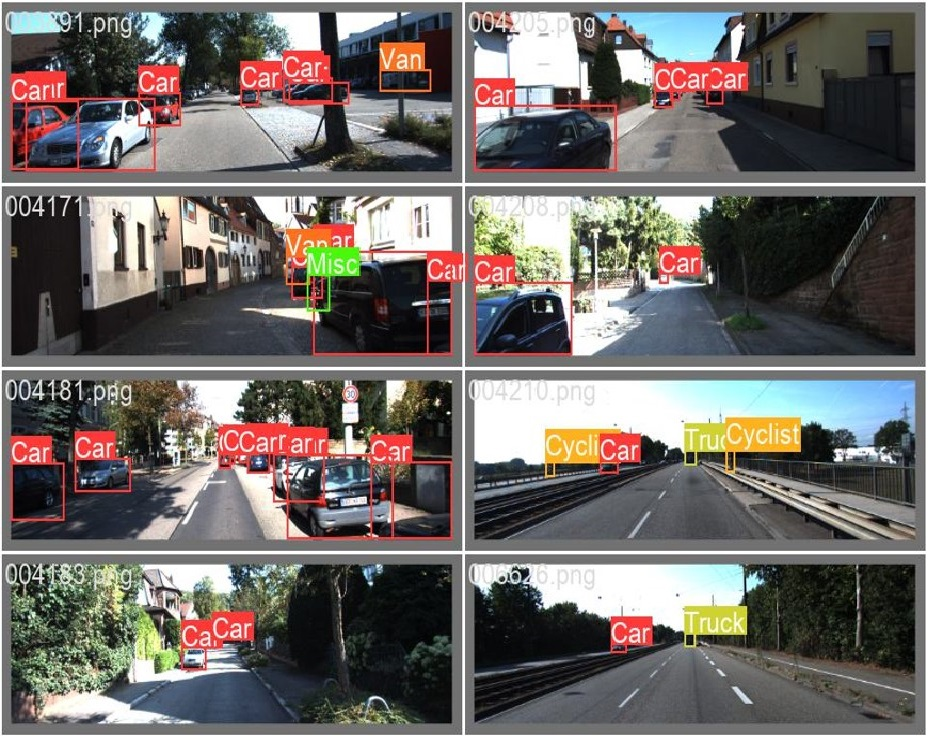
\includegraphics[width=7.5cm]{./img/Validation_data.png} }}
    \qquad
    \subfloat[\centering Выходные данные]{{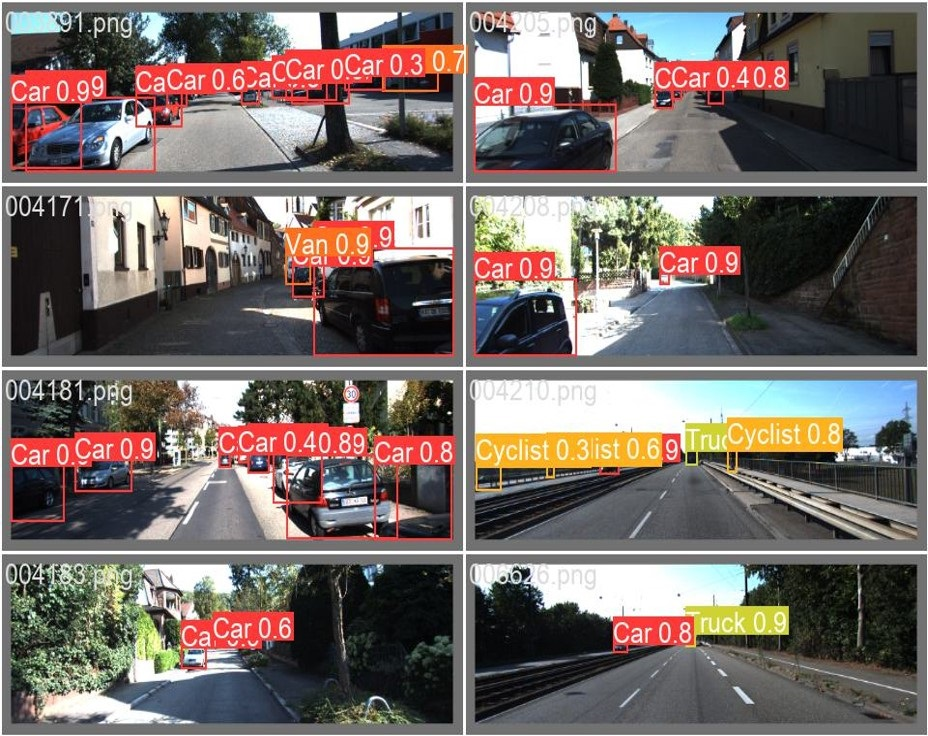
\includegraphics[width=7.5cm]{./img/Output_data.png} }}
    \caption{Сравнение валидационных и выходных данных}%
    \label{fig::ResultsCompare}%
\end{figure}

Из сравнения двух сторон можно сделать несколько наблюдений:

\begin{itemize}

	\item Модель успешно распознаёт и правильно классифицирует большинство объектов, 
	таких как автомобили и велосипедисты.
	\item Указанные уверенности для обнаруженных объектов в целом высоки, что 
	свидетельствует о надёжности детекции.
	\item Есть некоторые несоответствия, например, на одном из изображений модель 
	пометила лишние автомобили, что может указывать на возможные проблемы с точностью
	или с разнообразием данных в обучающем наборе.

\end{itemize}

В целом, результаты показывают, что обученная модель ведет себя довольно эффективно, 
обнаруживая и классифицируя объекты с высокой уверенностью, что является положительным
сигналом для систем автомобильного трекинга. Но также видно, что требуется дополнительная
настройка или обучение для устранения ошибок.